% !TeX encoding = UTF-8
% !TeX root = ../main.tex
% !TeX spellcheck = en_US
\chapter{Work}
\label{cha:work}

This chapter describes the experiments and approaches tried and implemented during the thesis. It should give a description about the decisions made and the problems occurred based on the decisions and implementation limitations.

\section{Extracting features}

The image feature were represented by \acf{HOG} (as described in \prettyref{sec:hog})

\section{Abstracting the feature computation}

One of the initial steps made was to find a way to represent a collection of extracted features (as taken from a part candidate or a query image). This should enable the precomputation of the image database and also create a similarity linkage right away into the stored database.

To fulfill these requirements, the decision goes to try to cluster the features with a k-means clustering (see \prettyref{sec:kmeans}) or a fisher vector representation (see \prettyref{sec:fisher}) based on a \acf{GMM} (see \prettyref{sec:gmm}).
\par
The initial experiments were used to detect if codebooks based on clustered features could be used to express similarities among different candidates. This was done by using the bicycle and car classes of the \ac{VOC2011} Image database \cite{Pascal2011}.
The clustering was initially done with 512, 1000 and 3000 k-means and 128, 256 and 384 \ac{GMM} clusters over all features extracted from the \ac{VOC2011} bicycle and car trainval image classes.
At this point all experiments were done by using normal \ac{HOG} and whiten \ac{HOG} (see \prettyref{sec:whitened_hog}) for performance comparison.
\par
The low-level \ac{HOG} implementation is provided by the Exemplar-SVM framework \cite{Malisiewicz2011}. This implementation produces a feature pyramid with $31$ dimensional features at different scales $S$.

\begin{equation}
S = \{s|s = \frac{1}{2^{0.1 * (i-1)}}; i \in \mathbb{N}; 1 \le i \le 100;\}
\end{equation}

For each level of the pyramid, the input image will be rescaled by the corresponding scale factor $s$, until no features could be extracted or the rescaled image contains less than 5 pixel per dimension.
\par
The calculated pyramid is then transfered in a list of feature vectors and their corresponding bounding boxes. This is done by combining the given features at each level of the pyramid into $5\times5$ grids and reshaping them into $775$ dimensional vectors.
As the experiments were executed with labeled bounding boxes, unnecessary features had to be removed from the list. This is achieved by specifying a pixel-wise boolean mask $M_p$ for the desired image regions. The mask will be transformed into a cell-wise $M_c$ at each scale $s$. This is done by a standard bicubic kernel convolution as in \eqnref{bicubic_kernel}.

\begin{equation}
k_x = \begin{cases}
(a+2)|x|^3-(a+3)|x|^2+1 & \text{for } |x| \leq 1 \\
a|x|^3-5a|x|^2+8a|x|-4a & \text{for } 1 < |x| < 2 \\
0                       & \text{otherwise}
\end{cases}
\label{eqn:bicubic_kernel}
\end{equation}

with $a=-0.5$ in the \MATLAB implementation\footnote{Implemented in the \textit{toolbox/images/images/imresize.m} file in the \MATLAB installation directory}. With this mask, all feature patches which are not fully covered by the mask were discarded.
\par
For the initial tests, a simple \acf{NN} approach with euclidean distances were used to compute the similarity between different codebooks.

This was done by selecting each labeled bounding box of each test image, computing the features $X$ (\ac{HOG} and whitened \ac{HOG}), assign them to the clusters by the corresponding centroids $C$ (either \ac{NN} in terms of k-means or by computing the fisher vector) and comparing it to the codebooks of the remaining image bounding boxes. The codebook values itself depend on the distances of the features to their corresponding centroids as described in \prettyref{eqn:codebook_calc}.

%TODO algorithm or formular???
%\begin{algorithm}
%	\KwIn{$X$: Features extracted from a bounding box, $C$: Cluster centroids}
%	\KwOut{$c$: codebook representing the given features}
%	\KwData{$D$: distance vector of each feature to its nearest centroid, $I$: assignment vector of each feature to its nearest centroid}
%	$D, I \gets \text{NearestNeighbourSearch}(X, C)$\;
%	
%	\ForEach{$d$ of $D$ and $i$ of $I$}{
%		$c_i \gets c_i + \frac{1}{d}$\;
%	}
%	\caption{Computing codebook from features}
%	\label{alg:codebook_calc}
%\end{algorithm}

\begin{align}
	I_j &= \arg \min_i ||X_j - C_i||_2 \\
	D_j &= \min_i ||X_j - C_i||_2 \\
	c_i &= \sum_{I_j = i} \frac{1}{D_j}
	\label{eqn:codebook_calc}
\end{align}

For a visual verification, the 15 nearest parts were shown aside to the query image. The distance between two different codebooks $c_1$ and $c_2$ was computed by the euclidean distance equation $||c_1-c_2||_2$.
%TODO beispiel bild
% searching for representative clusters (nn-iter)
For each query image, the most shared codebook dimensions and their respective patches were marked inside the images. It could be clearly seen that the patches with a comparable visual representation share the same cluster and (from a human perspective) seem to be representative for the chosen object class.
%TODO Bild mit markierung, oder auf vorheriges verweisen
To prove this assumption, an iterative \ac{NN} was implemented. It consists of several rounds, each executing a \ac{NN} search over the available patches and sorting the results. After each round, the most common codebook dimensions of the first $k$ patches were taken whilst the remaining ones were removed (set to zero) as described by \prettyref{alg:iterative_nn}.

\begin{algorithm}
	\SetKwProg{Fn}{Function}{}{end}
	\Fn{IterNearestNeighbour($q$ : query codebook, $R$ : remaining codebooks, k)}{
		\Repeat{no changes}{
			$D \gets \text{NearestNeighbourSearch}(R, q)$\;
			
			Sort $R$ based on $D$\;
			
			\tcc{$ij$ denotes dimension $i$ in codebook $j$}
			
			$S = \{i | \forall R_{ij} \ne 0; 0 < j < k\}$\;
			
			$R \gets R_{ij}$ set to $0$ if $i \notin S$\;
		}
		\Return{Sorted $R$}
	}
	\caption{Iterative \ac{NN}}
	\label{alg:iterative_nn}
\end{algorithm}

By using this algorithm, it could be shown that the most representative patches were assigned to the same clusters, as more similar objects are pulled together at each iteration.
%TODO bilder fuer verschiedene iterationen 

\par
% maintaining location information (parts)
As the reduction of several feature vectors to a single codebook for a whole bounding box eliminates the locational information, the implementation was extended to maintain some locational information by splitting the bounding box in several parts and computing a codebook for each of them. Afterwards, these codebooks are concatenated, which means that the size of a representative codebook for a whole bounding box is calculated by $numberOfParts * numberOfDimensions$. This change brought additional performance gains in terms of detecting similar parts, but also increased the memory usage significantly. During the rest of the experiments, the bounding boxes were either split into a two-by-two grid (as it seemed to be the best mix of performance gain and memory usage) or left complete for later comparisons.

\section{Scoring the part candidates}

% svm

As the direct comparison via a \ac{NN} approach did not provided the desired performance and also resulted in a time consuming task if the amount of codebooks increases, another approach was required. One possible solution for detecting similar vectors is a \ac{SVM} based classifier (for a more detailed description about \acp{SVM} see \prettyref{sec:svm}). In this particular case a C-SVC classifier was trained \cite{boser1992training} \cite{cortes1995support}.
%In this particular case a one-vs-call classifier was used. In this type only one classifier is trained to determine if a given vector is part of one class or part of all other possible classes.
The positive class is represented by the query codebook, whilst all other classes are represented by a previously collected list of codebooks. To generate this list, a set of sliding windows were calculated for each image in the database based on \algref{calc_windows}.

\begin{algorithm}
    \KwIn{$I$: image}
    \KwOut{calculated windows}
    $w_I \gets \text{width of }I$\;
    $h_I \gets \text{height of }I$\;
    $S \gets \{s^2 | s \in \mathbb{N}, s \le 10 \}$\;
    $x \gets \{1, 11, 21, 31,\dots, w_I\}$\;
    $y \gets \{1, 11, 21, 31,\dots, h_I\}$\;
    \Repeat{$w_w >= w_I$ or $h_w >= h_I$ or no elements left in $S$}{
        $currentScale \gets \text{next element of }S$\;
        $w_w \gets 32 * currentScale$\;
        $h_w \gets 32 * currentScale$\;
        
        \ForEach{Combination $x_i, y_i$ of $x$ and $y$}{
            Add window $x_i, y_i, x_i + w_w, y_i + h_w$ to the list\;
        }
    }
    \caption{Calculation of sliding windows}
    \label{alg:calc_windows}
\end{algorithm}

With this list, all feature patches are assigned to these windows where their center is placed in. For each window, a codebook is calculated by \eqnref{codebook_calc}. The resulting list of codebooks is stored and loaded during the \ac{SVM} training and used as the negative training set. The \ac{SVM} training was done by the libsvm library \cite{Chang:2011:LLS:1961189.1961199} by using the \texttt{svmtrain} function. The parameters for the training are the same as for the ExemplarSVM library \cite{Malisiewicz2011} (see \tabref{libsvm_train_params}).

\begin{table}
    \begin{tabular}{|l|l|}
        \hline
        \textbf{Parameter} & \textbf{Value} \\ 
        \hline
        SVM-Type           & C-SVC \\ 
        \hline
        Kernel-Type        & Linear ($u^T*v$) \\ 
        \hline
        Cost ($C$ of C-SVC)  & $0.01$ \\ 
        \hline
        Weight of positive sample ($weight*C$) & $50$ \\ 
        \hline
    \end{tabular}
    \caption{libsvm parameters}
    \label{tab:libsvm_train_params}
\end{table}

Other assignment methods were also evaluated, including multi assignments like assigning a feature to every window were a corner is located in, or to every window which contains a minimum amount of the patch (e.g. 30\% of its area). These approaches did not provide enough performance gain in comparison to the computational overhead. Another approach was the usage of the bottom right corner, which obviously led to the fact that the detection candidates were slightly shifted to the bottom right compared to an optimum detection. 

In the first place, the classification function provided by libsvm\footnote{\texttt{svmpredict(\dots)}} was used. With an increasing amount of codebooks which have to be classified by the \ac{SVM}, the function toked a big part of the computation time. By replacing the function with the \MATLAB implementation ($codebooks * (svm_{vectors}^T * svm_{coefficents}) - svm_{\rho}$) (see \prettyref{lst:matlab_svm_predict}), the computation time could be reduced from approximate 150 seconds to 3 seconds with 250,000 codebooks (5,000 windows in 50 images).


\begin{lstlisting}[caption={\MATLAB variant of svmpredict},label=lst:matlab_svm_predict]
weights = m.SVs' * m.sv_coef;

if size(codebooks, 2) == size(weights, 1)
    scores = codebooks * weights - m.rho;
else
    scores = codebooks' * weights - m.rho;
end
nans = isnan(scores);
debg('%d NaNs produced!', sum(nans))
scores(nans) = -999;
\end{lstlisting}

\section{Reducing the computational overhead}

% integral image
During the shift from the initial tests involving the usage of labeled bounding boxes to the actual requirement of finding parts inside of image databases, the amount of computational overhead increased significantly as it requires to compute sliding windows on each image in the database and their codebooks respectively.

Therefore the idea came up to precompute the codebooks and only load them at runtime for comparison. One solution would be to compute a set of possible windows and their codebooks. At query time the best matching window ratios could be loaded and compared to the query codebook. Unfortunately was the performance dramatically decreased with this approach.

The second solution was to create integral images based on codebooks. Integral images were described by Viola and Jones in 2001 \cite{viola2001rapid}. Such images are created by summing up all pixel values from the top left to the bottom right (or any other diagonal direction). The advantage of this approach is the possibility to compute a sum value for a rectangular area by summing and subtracting the values of the four corners as described in \figref{integral_image}. 

\begin{figure}
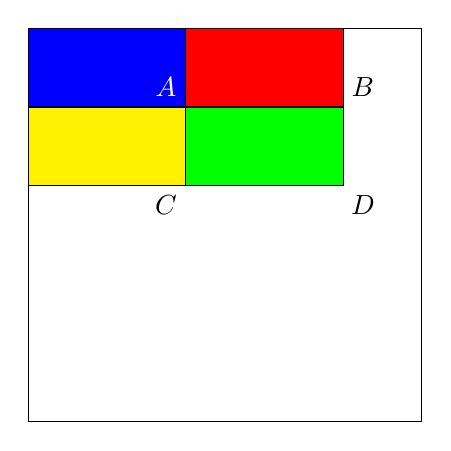
\begin{tikzpicture}
\draw (0,0) rectangle (5,5);
\draw[fill=blue] (0,5) rectangle (2,4);
\draw (1.75, 4.25)  node[white] {$A$};
\draw[fill=red] (2,5) rectangle (4,4);
\draw (4.25, 4.25)  node{$B$};
\draw[fill=yellow] (0,4) rectangle (2,3);
\draw (1.75, 2.75)  node{$C$};
\draw[fill=green] (2,4) rectangle (4,3);
\draw (4.25, 2.75)  node{$D$};
\end{tikzpicture}
\caption[Sum of area in integral image]{The sum of all values in the green area could be computed by $A+D-(C+B)$. $A$ is the sum of all pixels in the blue area, $B$ the sum of the pixels in the blue and the red areas, $C$ the sum of all pixels in the blue and yellow areas, $D$ of the green, red, blue and yellow respectively}
\label{fig:integral_image}
\end{figure}

The difference to \cite{viola2001rapid} is that one pixel at a time is represented by a complete codebook, therefore an integral image per codebook dimension has to be computed. The source image is created by adding the inverse distance of each feature patch center to its nearest cluster centroid to the corresponding codebook dimension. Afterwards, a cumulative sum over the two image axes is computed. The benefit of using integral images is that at runtime, every possible window could be computed by four reads (the corners), one sum and two subtractions between the codebooks. This reduced the computational time at the query stage to 1-2 seconds with a $500\times375$ image, 1000 codebook dimensions and 5000 windows with a 2-by-2 grid.

The downside is the memory usage, which increased dramatically. For example, a $500 \times 375 \times 1000$ integral image requires with the double datatype at least 1.4 gigabytes of data (without any meta information stored aside by matlab). The 50 images test database required therefore at least 70 gigabytes of RAM storage during the query. This also led to the problem of the time required to load the whole database. By storing it in the \MATLAB 7.3 file format, which effectively is a slightly modified HDF5 \cite{hdf5}, the program requires in average 900 seconds to load the whole database from a network shared filesystem.

This method also enabled the extraction of the query codebook from an image contained in the database without any feature or codebook computations. The reduced computational effort during the query phase consist therefore in extracting the query codebook from the database, training of the \ac{SVM}, calculating the sliding windows, extracting the codebook for each window in each image and scoring the codebooks by the trained \ac{SVM}.
% no libsvm classify

\section{Optimizing the score output}

%TODO non max suppression

The experiments showed that the \ac{SVM} output does not provide a clear separation threshold to identify positive candidates over all images in the database. The scores varied between -2 and 1 for the best matching candidates. As the candidates were most of the time correctly ordered by their visual similarity to the query image, this would not be a problem under the assumption that every image contain at least one area which is similar to the query image part. In this case, the scores could be normalized at an image level, which means that significant higher scores compared to the arithmetic mean are considered positive, whereas scores near the mean or lower are considered negative. %TODO bild von score histogram
As one will see in \figref{score_histogram}, this would fit for the most pictures used during the testing. The majority of windows is located at the same score, whereas windows with a score above the mean are closely located to the desired image part.
% gaussian fit + rho adjust
This additional normalization obviously increases the computation effort as it had to be done separately for each image in the database (after computing the scores for each window in the image). Therefore an approximation was applied by normalizing the scores in relation to the query image. To normalize the scores, a Gaussian curve is fitted onto the scored query image windows. By shifting the curve by $3\sigma$ into the direction of the highest scores, the relevant (positive) scores where pulled up near to one, whereas the negative scores get pushed down to zero. The resulting curve is then applied to all scores. This approximated normalization enabled us to produce comparable scores and therefore exclude whole images from the query results.

Another approach was to create a per image $svm_\rho$ value (comparable to the mean threshold) to orientate the scores at a common center point, but it turned out that the effort were to high compared to the performance gain.

After the score computation and normalization, a non maximum suppression was applied to minimize the output of similar, near located windows.
During the experiments, two non maximum suppression techniques were used and evaluated.

The first one is constructed by the union of the areas to compare (\ref{eqn:nonmax_union})

\begin{equation}
\frac{\text{area}(A \cap B)}{\text{area}(A \cup B)}
\label{eqn:nonmax_union}
\end{equation}

This technique computes the ratio between the common and total area of two bounding boxes $A$ and $B$. If this ratio has a value higher than $0.5$, the bounding box $B$ would be removed from the result list.

The second technique is based on \eqnref{nonmax_min}. This variant removes much more bounding boxes if they are enclosed by others, as only the area of smallest bounding box is used as the denominator. The previous technique removes only enclosed bounding boxes which are at least half as big as their enclosing boxes.

\begin{equation}
\frac{\text{area}(A \cap B)}{\min(\text{area}(A), \text{area}(B))}
\label{eqn:nonmax_min}
\end{equation}

The current algorithm produced the best results with the second technique, as it reduces the repetition of many positive windows showing only a single bicycle wheel. As they would not cover 50\% of the window enclosing the whole bicycle, they appear as new matches in the result list by using the first technique. Depending on the query image, it could be useful to switch between the suppression techniques as it could be desired to get smaller matches enclosed by a bigger one (for example children in front of their parents).

\section{Reducing the memory usage}

After optimizing the detection performance, the memory usage was still to high to provide an useful alternative/boosting algorithm to the ExemplarSVM algorithm. To minimize the memory overhead, several approaches were developed and evaluated. These approaches include different storage mechanisms as kd-tree, spares matrices or plain index-value pairs and also different search and reconstruction strategies.

\subsection{Sparse matrices}

One approach is to use sparse matrices as provided by the \MATLAB framework\footnote{\url{https://de.mathworks.com/help/matlab/ref/sparse.html}}. The usage seemed to be very promising, as partial inspections of the integral images showed that approx. 70\% of the cells in a $512\times500\times375$ matrix are filled with zeros.

It showed that the \MATLAB implementation of sparse matrices is restricted to two-dimensional matrices, it is therefore required to reduce the amount of dimensions of the matrix at store time and restore the original format at runtime, or transform the required coordinates into a single index. As the internal representation of an image consists of four matrix dimensions (scale range, codebook dimensions, width, height), a matrix will be transformed into a matrix of the form $CB \times N$ whereas $CB$ is the amount of codebook dimensions and $N$ the product of the image width, height and number of scale ranges included in this matrix (usually one per saved \MATLAB file). The corresponding source code could be seen in \lstref{storage_method_sparse} in line 171. The variable \verb|si| represents the current scale ranges which will be saved. A complete reconstruction to the original, internal representation could be done with \lstref{reconstruct_sparse_matlab}. This is done by converting the sparse matrix into a full matrix containing the zero values. The new matrix is then reordered into its original four dimensional representation.

\begin{lstlisting}[firstnumber=165,caption={Sparse storage method (get\_codebook\_integrals.m)},label=lst:storage_method_sparse]
I2 = I(si, :, :, :);
Is = size(I2);
integrals(si, fi).I_size = Is;
if params.naiive_integral_backend
    integrals(si, fi).I = I2;
elseif params.integral_backend_matlab_sparse
    integrals(si, fi).I = sparse(squeeze(I2(:, :, :)));
\end{lstlisting}

\begin{lstlisting}[firstnumber=29,caption={Sparse reconstruction by \MATLAB (getCodebookIntegrals.m)},label=lst:reconstruct_sparse_matlab]
I = full(integralImg.I);
I = reshape(I, integralImg.I_size);
\end{lstlisting}

The matrices are stored in a \MATLAB file with the 7.3\footnote{A comparison table could be found at \url{https://de.mathworks.com/help/matlab/ref/save.html\#input_argument_version} (visited on 10/12/2015)} file format (required to store variables with more than two gigabytes of data).
For example the representation of the pascal image \textit{2007\_008932.jpg} containing feature patches with a maximum size of $86\times86$ pixels and 512 codebook dimensions results in a total \ac{RAM} size of 768,001,438 bytes (or 732.4 megabytes). The saved \MATLAB file occupies 6,325,415 bytes (6 megabytes) of disk space.
Stored as a sparse matrix the data is reduced to 423,905,670 bytes (404.3 megabytes or 55\%) in \ac{RAM}. After saving to a file, a size of 22,612,163 bytes (21.6 megabytes) still remains. Compared to the na\"{\i}ve (saving the matrices as is) storage method it requires 16,286,748 bytes more (15.5 megabytes or 357\%) disk space. The reason for this storage overhead could probably be found in the mandatory compression which comes with file formats greater or equal to version 7.0. For the na\"{\i}ve format, the compression can benefit from the low entropy coming from the high amount of zeros which exists in a sequential ordering. In contrast to the sparse variant, which have to compress multiple lists of coordinates and their corresponding values. Besides the fact that disk storage is a cheap resource nowadays, it also affects the loading time as more data has to be loaded. Although the decompression time could be reduced as a much lesser compression ratio was achieved. Together with the additional matrix reconstruction described above, a small speedup was still achieved whilst the memory usage was reduced by 50\%.

\subsection{Reconstructing from changing points}

As the internal representation is based on integral images, additional information can be interfered from on specific points in the matrix. Integral images are constructed by summing up values from the top left to the bottom right. This means that as long as no further points exists in the source image, the most current value is carried on until the next point is found. The example in \figref{integral_image_interference} shows and describes the behavior. As one can see, the minimum required information to construct a full integral image are the values at the points $(2,9)$, $(3,4)$, $(5,6)$ and $(5,8)$. In contrast to the sparse matrix approach, only 4 points have to be stored compared to 58 points.

Obviously the computation effort during the query search increases as the integral image would had to be computed at runtime. By sorting the points according to the sum of their coordinate values, the computation overhead could be reduced as the amount of cells which have to be summed up decreases with every point processed.
%TODO timings + memory

%\begin{lstlisting}[firstnumber=229,caption={Coordinate based storage method (get\_codebook\_integrals.m)},label=lst:storage_method_coordinate]
%[cb, x, y] = ind2sub(Is(2:end), find(remaining));
%coords = [x, y, cb];
%
%sum_values = coords(:, 1) + coords(:, 2);
%[~, idx] = sort(sum_values);
%coords = coords(idx, :);
%scores = scores(idx, :);
%
%integrals(si, fi).coords = coords;
%integrals(si, fi).scores = scores;
%\end{lstlisting}

To find a trade-off between low memory usage and computation effort, another approach came up. In this approach every changing value in the integral image is stored instead of the original values. In the current example the points $(2,9)$, $(3,4)$, $(3,9)$, $(5,6)$, $(5,8)$ and $(5,9)$ would be selected. By storing the additional points, which were created at the intersection points of the original ones, we are able to reconstruct the full matrix by taking the list of points, sorting them by the sum of their coordinates and writing one point at a time from its position to the bottom right. In the current example the list would be sorted as \mathlist{(3,4), (5,6), (2,9), (3,9), (5,8), (5,9)}. In the first step the point $(3,4)$ would be selected and its value ($2$) would be written to the bottom right as shown in \figref{integral_image_interference2:point1}. The second step selects point $(5,6)$ and write its value $5$ in the same way as before.
This technique will be applied to all points in the list until the integral image is fully reconstructed.
The speed up comparing to the previous approach is based on the fact that no memory read from any cell has to be made and no arithmetic instruction has to be executed. The limiting factor in this case is ability to write values fast at specific positions in \ac{RAM}.
%TODO timings + memory

\begin{figure}
\begin{subfigure}{.5\textwidth}
    \resizebox{\textwidth}{\textwidth}{
        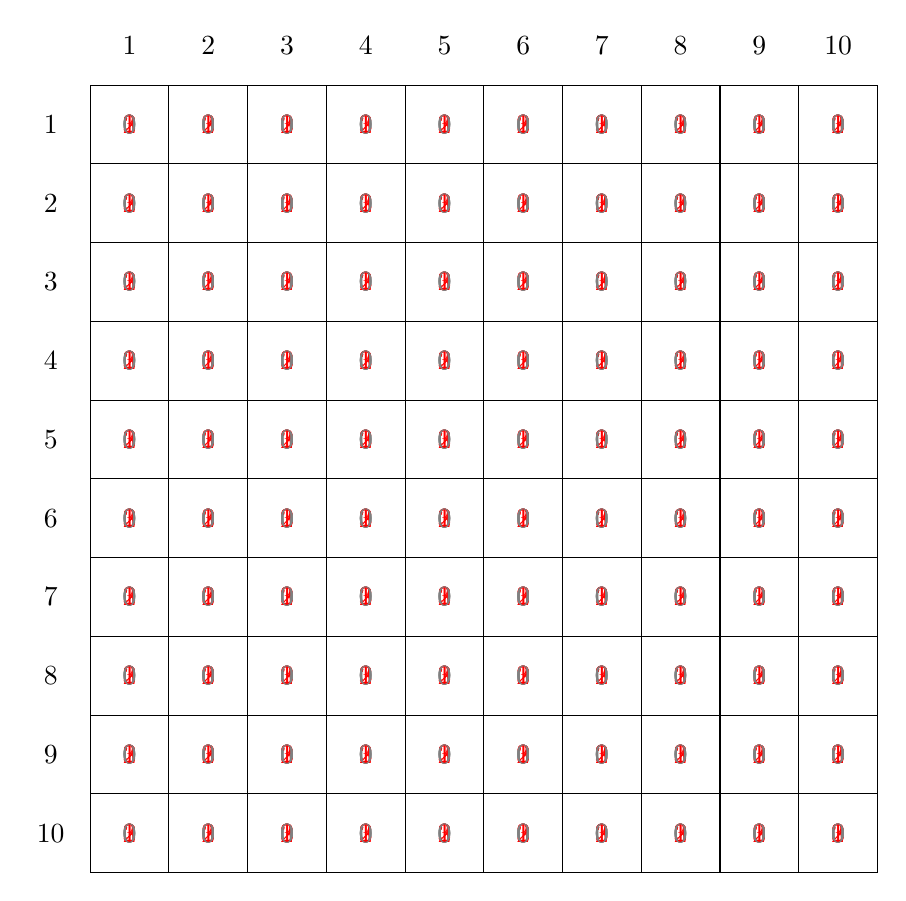
\begin{tikzpicture}
        \foreach \x in {1,...,10} {
            \draw (\x + 0.5, 11.5) node {\x};
        }
        \foreach \y in {10,...,1} {
            \draw (0.5, 11.5 - \y) node {\y};
        }
        \foreach \x in {1,...,10} {
            \foreach \y in {1,...,10} {
                \draw (\x, \y) rectangle (\x +1, \y +1);
                \ifnumequal{\x}{5}{
                    \ifnumequal{\y}{5}{
                        \draw[color=red] (\x +0.5, \y +0.5) node {3};
                    }{
                        \ifnumequal{\y}{3}{
                            \draw[color=red] (\x +0.5, \y +0.5) node {2};
                        }{
                            \draw[color=gray] (\x +0.5, \y +0.5) node {0};
                        }
                    }
                }{
                    \ifnumequal{\x}{2}{
                        \ifnumequal{\y}{2}{
                            \draw[color=red] (\x +0.5, \y +0.5) node {1};
                        }{
                            \draw[color=gray] (\x +0.5, \y +0.5) node {0};
                        }
                    }{
                        \ifnumequal{\x}{3}{
                            \ifnumequal{\y}{7}{
                                \draw[color=red] (\x +0.5, \y +0.5) node {2};
                            }{                    
                                \draw[color=gray] (\x +0.5, \y +0.5) node {0};
                            }
                        }{
                            \draw[color=gray] (\x +0.5, \y +0.5) node {0};
                        }
                    }
                }
            }
        }
        \end{tikzpicture}
    }
    \caption{Source image}
    \label{fig:integral_image_interference:source_image}
\end{subfigure}%
\begin{subfigure}{.5\textwidth}
    \resizebox{\textwidth}{\textwidth}{
        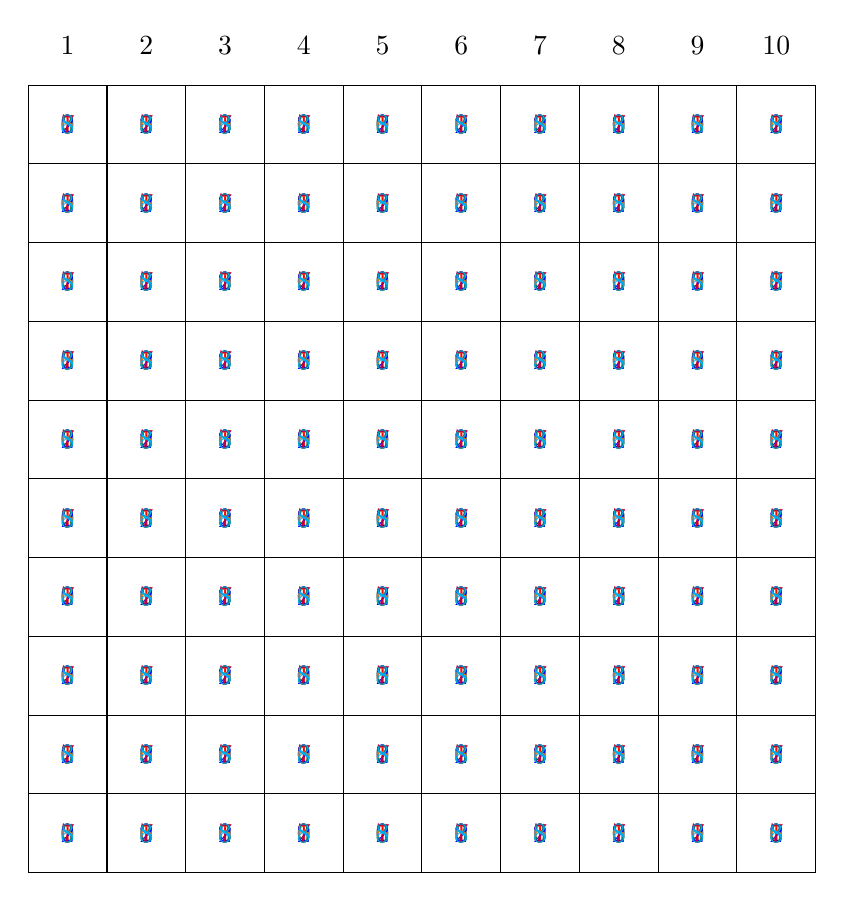
\begin{tikzpicture}
        \foreach \x in {1,...,10} {
            \draw (\x + 0.5, 11.5) node {\x};
        }
        \foreach \x in {1,...,10} {
            \foreach \y in {1,...,10} {
                \draw (\x, \y) rectangle (\x +1, \y +1);
                \ifnumcomp{\x}{<}{2}{
                    \draw[color=gray] (\x +0.5, \y +0.5) node {0};
                }{
                    \ifnumcomp{\x}{<}{3}{
                        \ifnumcomp{\y}{>}{2}{
                            \draw[color=gray] (\x +0.5, \y +0.5) node {0};
                        }{
                            \draw[color=red] (\x +0.5, \y +0.5) node {1};
                        }
                    }{
                        \ifnumcomp{\y}{>}{7}{
                            \draw[color=gray] (\x +0.5, \y +0.5) node {0};
                        }{
                            \ifnumcomp{\y}{>}{2}{
                                \ifnumcomp{\x}{<}{5}{
                                    \draw[color=blue] (\x +0.5, \y +0.5) node {2};
                                }{
                                    \ifnumcomp{\y}{>}{5}{
                                        \draw[color=blue] (\x +0.5, \y +0.5) node {2};
                                    }{
                                        \ifnumcomp{\y}{>}{3}{
                                            \draw[color=orange] (\x +0.5, \y +0.5) node {5};
                                        }{
                                            \draw[color=purple] (\x +0.5, \y +0.5) node {7};
                                        }
                                    }
                                }
                            }{
                                \ifnumcomp{\x}{<}{5}{
                                    \draw[color=teal] (\x +0.5, \y +0.5) node {3};
                                }{
                                    \draw[color=cyan] (\x +0.5, \y +0.5) node {8};
                                }
                            }
                        }
                    }
                }
            }
        }
        \end{tikzpicture}
    }
    \caption{Integral image}
    \label{fig:integral_image_interference:integral_image}
\end{subfigure}%
\caption{The source image in \subref{fig:integral_image_interference:source_image} contains values at the positions $(2,9)$, $(3,4)$, $(5,6)$ and $(5,8)$. As shown in \subref{fig:integral_image_interference:integral_image} their values expand to the bottom right. Even if the amount of zero values decreased, the matrix contain still a high percentage of repetitions.}
\label{fig:integral_image_interference}
\end{figure}

\begin{figure}
\begin{subfigure}{.5\textwidth}
    \resizebox{\textwidth}{\textwidth}{
        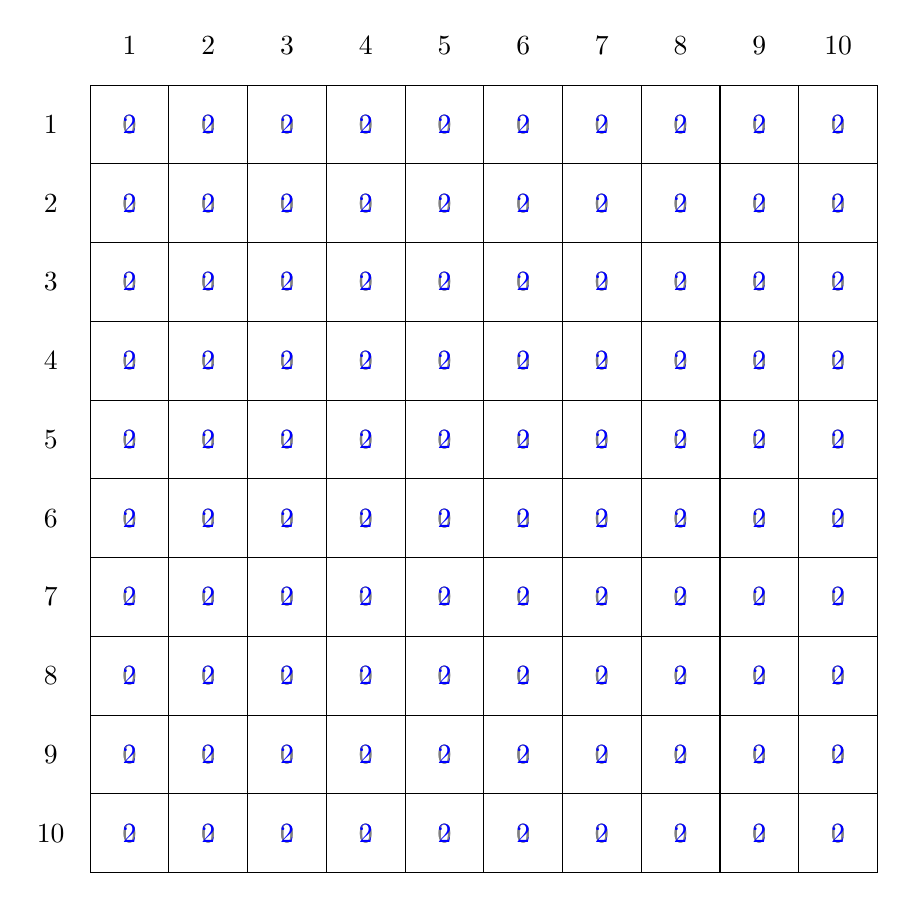
\begin{tikzpicture}
        \foreach \x in {1,...,10} {
            \draw (\x + 0.5, 11.5) node {\x};
        }
        \foreach \y in {10,...,1} {
            \draw (0.5, 11.5 - \y) node {\y};
        }
        \foreach \x in {1,...,10} {
            \foreach \y in {1,...,10} {
                \draw (\x, \y) rectangle (\x +1, \y +1);
                \ifnumcomp{\x}{<}{3}{
                    \draw[color=gray] (\x +0.5, \y +0.5) node {0};
                }{
                    \ifnumcomp{\y}{>}{7}{
                        \draw[color=gray] (\x +0.5, \y +0.5) node {0};
                    }{
                        \draw[color=blue] (\x +0.5, \y +0.5) node {2};
                    }
                }
            }
        }
        \end{tikzpicture}
    }
    \caption{Reconstructing point $(3,4)$}
    \label{fig:integral_image_interference2:point1}
\end{subfigure}%
\begin{subfigure}{.5\textwidth}
    \resizebox{\textwidth}{\textwidth}{
        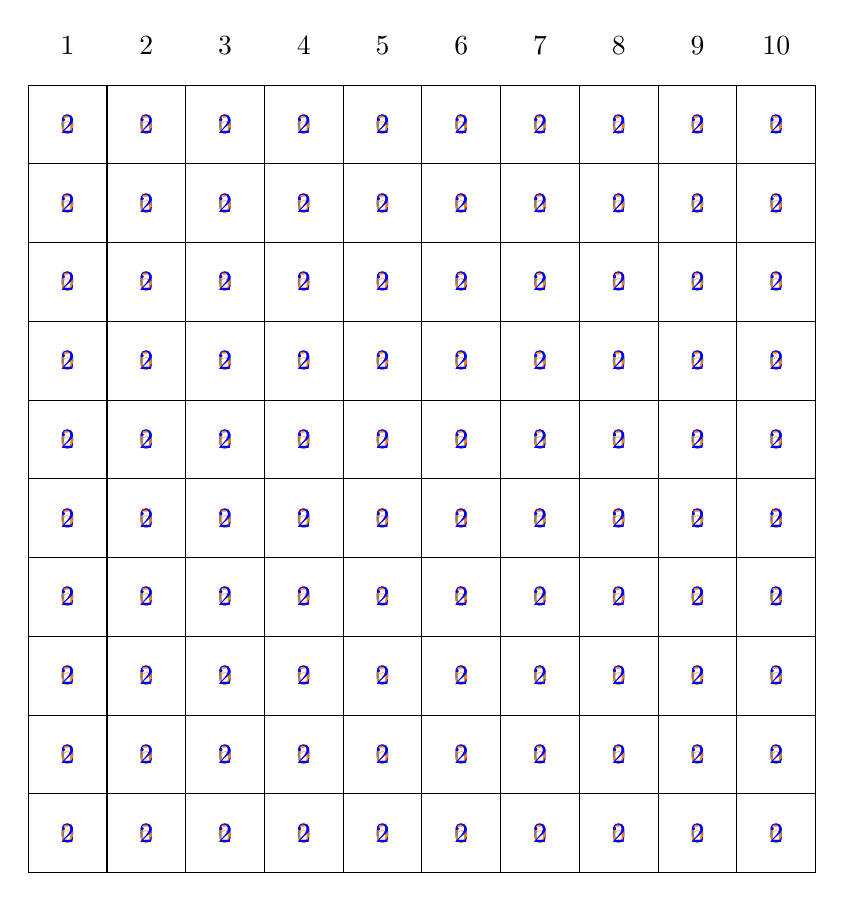
\begin{tikzpicture}
        \foreach \x in {1,...,10} {
            \draw (\x + 0.5, 11.5) node {\x};
        }
        \foreach \x in {1,...,10} {
            \foreach \y in {1,...,10} {
                \draw (\x, \y) rectangle (\x +1, \y +1);
                \ifnumcomp{\x}{<}{3}{
                    \draw[color=gray] (\x +0.5, \y +0.5) node {0};
                }{
                    \ifnumcomp{\y}{>}{7}{
                        \draw[color=gray] (\x +0.5, \y +0.5) node {0};
                    }{
                        \ifnumcomp{\y}{<}{6}{
                            \ifnumcomp{\x}{>}{4}{
                                \draw[color=orange] (\x +0.5, \y +0.5) node {5};
                            }{
                                \draw[color=blue] (\x +0.5, \y +0.5) node {2};
                            }                                                    
                        }{
                            \draw[color=blue] (\x +0.5, \y +0.5) node {2};
                        }                      
                    }
                }
            }
        }
        \end{tikzpicture}
    }
    \caption{Reconstructing point $(5,6)$}
    \label{fig:integral_image_interference2:point2}
\end{subfigure}%
\caption{Reconstructing integral image from intersection points}
\label{fig:integral_image_interference2}
\end{figure}

The fourth approach tried to achieve an additional reduction of the writing cycles. This is done by storing additional points, which are selected by scanning the integral image row by row. Each time a value change is detected, the point is added to the list. In the example the complete list would be noted as \mathlist{(3,4), (3,5), (3,6), (5,6), (3,7), (5,7), (3,8), (5,8), (2,9), (3,9), (5,9), (2,10), (3,10), (5,10)}. In the reconstruction phase, the algorithm jumps at the first point for each row and writes its value to the right until he reaches the next point in the list. Now the new value is written to right until the next point is reached and so forth.
%TODO timings + memory

The fifth approach skips the reconstruction completely and tries to find any value by searching in the list of intersection values from the third approach. In the initial implementation, the scores were stored aside to their x, y and codebook dimension coordinates ($img_x$, $img_y$ and $img_{codebook}$ respectively). The actual search consisted of three steps. In the first step, all coordinates and values are selected which correspond to the lower or equal x values compared to the query x value ($query_x$). Within the subset all values belonging to $img_y \le query_y$ are selected. The resulting subset is scanned from lower to higher coordinates (sorted by $img_x$, $img_y$ and $img_{codebook}$) and will fill a codebook based on the $img_{codebook}$ and score values.

As one may notice this represents more or less multiple linear searches, which has to be done by every requested codebook at a specific point. To speedup the search a binary searching algorithm based on kd-trees were implemented. %TODO binary search, kd-tree
Instead of filtering by the x and y coordinates first and filling the codebook with the last changed values, the filtering for this approach was reversed. Every integral image is represented by as many kd-trees as codebook dimensions exist. If one codebook dimension is never used throughout the while image, the corresponding tree will be empty. Each of the remaining trees consist of two matrices. The first matrix contains three rows with as many columns as unique x coordinates for this codebook dimension exist. The first row contains the current x coordinate, the second the starting index for the second matrix and the third row the end index for the second matrix. The second matrix consists of two rows. One containing all y coordinates and the other all scores.

When searching a value for a specific codebook dimension at a specific point, the kd-tree which corresponds to the codebook dimension is selected. Within the first matrix the highest x value lower or equal to $query_x$ is searched and the second matrix is cut to the start and end indices extracted from the first matrix. Within this smaller matrix the highest y value lower or equal to $query_y$ is searched and the corresponding score is used as the codebook dimension value. Both searches can be done by a binary search approach in $O(\log_2 N)$. Additionally, most of the searches will be canceled early, as either the codebook dimension is empty, the $query_x$ is outside of the x values or $query_y$ is outside of the y values. %TODO nachweis????
%TODO timings + memory

%\begin{lstlisting}[firstnumber=179,caption={KD-Tree storage method (get\_codebook\_integrals.m)},label=lst:storage_method_kdtree]
%remaining = I2 ~= 0;
%
%I2 = I2(remaining);
%scores = I2(:);
%if params.use_kdtree
%    [cb, x, y] = ind2sub(Is(2:end), find(remaining));
%    % sort order: y x cb
%    coords = [cb, x, y];
%    cb = unique(cb);
%    cblen = length(cb);
%    if cblen > 0
%        tmptree = alloc_struct_array(cblen, 'x', 'y');
%        parfor ci=1:cblen
%            dim = cb(ci);
%            if ci == 1 || ci == cblen || mod(ci, 100) == 0
%                debg('[%4d/%04d] Dimension %d', ci, cblen, dim);
%            end
%            cs = coords(:, 1) == cb(ci);
%            x = coords(cs, 2);
%            y = coords(cs, 3);
%            s = scores(cs);
%            ux = unique(x);
%            data2 = zeros([length(ux) 3], 'uint32');
%            data2(:, 1) = ux;
%            data3 = zeros([length(y) 2]);
%            from = 1;
%            to = 0;
%            for xi=1:length(ux)
%                xs = x == ux(xi);
%                sxs = sum(xs);
%                if sxs
%                    to = to + sum(xs);
%                    data3(from:to, 1) = y(xs);
%                    data3(from:to, 2) = s(xs);
%                    data2(xi, [2 3]) = [from, to];
%                    from = to+1;
%                end
%            end
%            tmptree(ci).x = data2;
%            tmptree(ci).y = data3;
%        end
%        tree = alloc_struct_array(Is(2), 'x', 'y');
%        tree(cb) = tmptree;
%    else
%        tree = alloc_struct_array(Is(2), 'x', 'y');
%    end
%
%    %tree = create_kd_tree(cb, tree);
%    integrals(si, fi).tree = tree;
%\end{lstlisting}

% kd - tree
% sparse matrix
% overwrite
% sum

\section{The framwork}
